% !TeX root = ../main.tex

% Implementation
% Explain all low-level implementation level details
\chapter{Implementation}\label{chapter:implementation}
This chapter will review low-level implementation details and explain what we had to do to get the reproducer working.
Firstly, we will talk about our additions to the verifier.
Then, we will discuss our Python program and explain the functionality of the two classes we designed.
Finally, we will review cases where the verifier might not work as expected.

\section{Additions to the Focaccia}
Focaccia is a full-fledged verifier that can be used to find bugs in emulators that stem from the wrong implementation of instructions.
However, because it was designed as a verifier, it lacks some useful features that would have helped the reproducer.
In this chapter, we will go over our additions to amend this.

Firstly, the original verifier would not return the actual state of the program before the execution of an instruction.
Naturally, this made it quite challenging to know what was inside the memory and registers.
We patched the verifier to return the snapshot of the program.

Our second addition was to the symbolic execution part of the verifier.
The symbolic expressions that the verifier can isolate are quite helpful.
It can return the following values from a given symbolic expression:
\begin{itemize}
    \item Symbolic expressions of the used and changed memory addresses
    \item A list of used registers
\end{itemize}
Both of these outputs are helpful since we can see which registers need to be restored and which memory locations need which values.
If we could change anything without considering the underlying hardware mechanisms like paging, permissions, and the actual location of the program in the memory, this might have been enough.
However, since this is not possible within this project's scope, we decided to allocate space in the data section and use it for memory.
This meant we needed to find the registers used explicitly for addressing the memory and change their values to point to the addresses in the data section.

We made this by adding a function to the symbolic execution program to evaluate any given expression except a register.
This meant that given a symbolic expression that points to an address, we could extract the used registers.
Then, we can be sure that these registers address memory and handle them as such.

The same mechanism also works for the stack.
We filter the symbolic expressions that point to memory for the stack pointer and assess whether they were used in the stack.

\section{Python Classes}
Since we were extending the verifier, we used the same programming language it was implemented in, namely Python.
Our reproducer is made up of two classes.
The first one, which is target agnostic, is called ReproducerEntry.
This class extracts information from the snapshot and the symbolic expressions.
The second class is called x86Reproducer.
As the name suggests, this class is x86 architecture-specific and is tasked with producing assembly instructions for its architecture.
The flow of data can be seen in figure \ref{fig:rep_ent}.
As the figure suggests, ReproducerEntry splits the snapshot using the symbolic expression and sets the x86Reproducer with the necessary values.
After this, the x86Reproducer prints the assembly code.

\begin{figure}[ht]
    \centering
    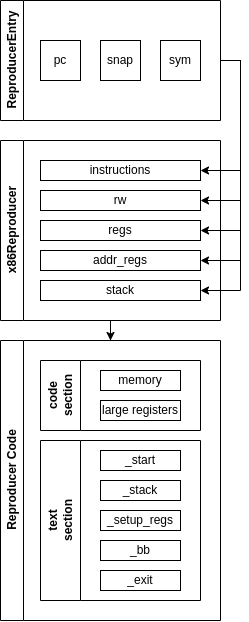
\includegraphics[width=0.5\linewidth]{figures/rep_ent}
    \caption{Flow of the reproducer including the ReproducerEntry and x86Reproducer classes.}
    \label{fig:rep_ent}
\end{figure}

\subsection{ReproducerEntry}
The backbone of our reproducer is the ReproducerEntry class.
It lets us find all of the necessary data using the snapshot and the symbolic expressions.
The main functionality of this class is shown in figure \ref{fig:rep_ent}, but we will go over the details:

\begin{itemize}
    \item get\_instructions:
    This function returns a list of instructions that make up the erroneous basic block.
    These instructions are received from only the symbolic expression.
    \item get\_rw\_addr:
    This function returns a dictionary of reads that will happen during the execution of the basic block and the writes that will happen as a result.
    Each entry is for a single byte; its key is the address.
    The reads keep the original values, while the writes are initialized with zeros.
    \item get\_regs:
    This function returns the dictionary of registers that are needed for the execution of the basic block.
    \item get\_addr\_regs:
    This function also returns a dictionary of registers.
    However, these are dictionaries that were only used for addressing memory.
    Moreover, the values of these dictionaries are not the register's values but the actual address they were used to point to.
    \item get\_stack:
    This function returns two values.
    Firstly, it returns the number of bytes that were subtracted from the stack pointer (either due to push operations or just subtraction from the stack pointer).
    Secondly, it returns the values that were in the stack.
    If a particular value is unused, its place is filled with zeros.
\end{itemize}

As shown, the ReproducerEntry is a versatile class that can extract everything we need from the snapshot and the symbolic expression.

\subsection{x86Reproducer}
This class is the part that produces the assembly instructions.
It is specifically designed to produce x86 assembly.
It receives all the information from the ReproducerEntry and does not directly use the snapshot or the symbolic expression.

In the data section, we initialize the values using the register and read/write dictionaries.
In the text section, the basic block is combined with stack and register setup code along with start and exit stubs.
The stack setup only uses what was returned from the stack values, while the register setup uses both the regular register dictionary and the addresses register dictionary.

\section{Shortcomings}
When trying to understand the reproducer's shortcomings, it is essential to remember that it was designed as an add-on to the verifier, which in turn depends on Miasm to work correctly.
As mentioned, our reproducer has some shortcomings regarding special registers and instructions.
This section will review these cases and explain why they are difficult to deal with.

Two crucial points should be considered when explaining why it is not possible to replicate bugs perfectly.
First of all, computer programs run step by step.
Each step changes the program's state, writes values to memory, and changes registers.
However, these are not all of the changes.
When a program is running, stack frames are built or destroyed, new pages are added, permissions are updated, and data handled by the kernel are changed.

A program is more than just its address space.
When trying to understand bugs that stem from emulation, we need to keep in mind that the hardware in the background is also part of the program.
All of the aforementioned data must be changed to replicate the state perfectly.
The simplest method to set the state is to run the program until that exact point is reached.


The second point is the symbolic expressions.
They are good at showing state transitions and building a tree for the execution path.
Nevertheless, they are an abstraction and lack details that might point to the bugs.
They do show what instructions do, but they are all on a transactional level.
For example, a symbolic expression might show a read operation, but it does not necessarily show whether the read address was an IO port or it was on a page that did not exist.
Therefore, we use it to guide us in the best way we can.

\subsection{Shortcomings of the Reproducer}
The reproducer has managed to reproduce bugs and code snippets that generally use simpler instructions to do calculations.
However, there are some shortcomings regarding more complicated instructions that affect the program flow or some registers for controlling the hardware.
These limitations will be discussed in the following sections.

\subsubsection{Instruction Pointer}
In CPUs, the instruction pointer is used to select the next instruction which will be executed.
Normally each instruction increments it by that instruction's size.
However, some instructions like jump, call, and return change the instruction pointer arbitrarily.
When this happens, the program expects its execution to continue somewhere else.
In these cases, the execution path changes to a different location, making testing them difficult.

\subsubsection{Segment Registers}
These registers were designed to let the original x86 CPU address more than 64 KB of memory.
However, these are currently used for other purposes like thread-local storage and canary-based stack protection.
Since changing them is very error-prone and these types of registers do not target the class of bugs we are trying to replicate, we decided to ignore them.

\subsubsection{Return Address}
When building the stack for the erroneous basic block,  the stack was set by using the values directly from the original snapshot.
We push these values directly after the start section.
However, this means that the return address of the function is wrong.
It is either zero, if it is not used at all, or it is the original return address.
Both of these values are likely to crash the program if used to return from the start section, but since we directly use the exit system call, the return address has no effect on the program.

\subsubsection{Indirect Memory Access}
Although our program can find memory access using reads and writes, we only look for them in the registers.
This makes sense since we must use at least one register to address a memory location.
However, in cases where a memory location has a pointer to a different address, our program cannot recognize them, and it will copy the same value, meaning it would be pointing to an unknown location.

This cannot happen when the reproducer is used for a single instruction since the address must already be in the register.
If a basic block is used and this problem arises, the best way to deal with it is to run the reproducer on every single instruction.
This method should prevent bugs arising from indirect memory access in a single basic block. 

\subsection{Segmentation Faults}
As we have mentioned previously, the verifier cannot detect \ac{segfault}s because, without the state that comes after the \ac{segfault}, the verifier will fail.
Even though the previous state is enough to set the reproducer, it will not be detected therefore it cannot recreate the bugs.

This weakness can be solved by adding a \ac{segfault} error to the verifier that happens when the emulator log is shorter than expected.
In that case, the reproducer can theoretically produce a program that can trigger the same \ac{segfault}.

However, this is not as simple as it sounds.
This might not always work because some \ac{segfault}s happen on special cases like alignment of the data or permissions of the memory section.
Unfortunately, the reproducer is oblivious to these things, making it difficult to replicate them.

\subsection{Shortcomings of the Symbolic Execution Engine}
We have added this section here to mention that our project relies on the verifier to function, which in turn relies on the symbolic execution engine.
This means that if the symbolic execution engine has problems like unimplemented instructions, our reproducer also suffers.

We have tested our reproducer with many different programs and noticed that most instructions that should have caused the bugs were not implemented in Miasm.
This had multiple different effects on the reproducer.
Sometimes, instructions would be mistranslated, and sometimes, they would be missing.
There is no simple solution except to fix Miasm itself.
